% !Mode:: "TeX:UTF-8"
\chapter{非线性优化}
\label{cpt:6}
\begin{mdframed}  
	\textbf{主要目标}
	\begin{enumerate}[labelindent=0em,leftmargin=1.5em]
		\item 理解最小二乘法的含义和处理方式。
		\item 理解高斯牛顿法(Gauss-Newton)、列文伯格—马夸尔特方法(Levenburg-\\Marquadt)等下降策略。
		\item 学习Ceres库和g2o库的基本使用方法。
	\end{enumerate}
\end{mdframed} 

在前面几讲,我们介绍了经典SLAM模型的运动方程和观测方程。现在我们已经知道,方程中的位姿可以由变换矩阵来描述,然后用李代数进行优化。观测方程由相机成像模型给出,其中内参是随相机固定的,而外参则是相机的位姿。于是,我们已经弄清了经典SLAM模型在视觉情况下的具体表达。

然而,由于噪声的存在,运动方程和观测方程的等式必定不是精确成立的。尽管相机可以非常好地符合针孔模型,但遗憾的是,我们得到的数据通常是受各种未知噪声影响的。即使我们有高精度的相机,运动方程和观测方程也只能近似成立。所以,与其假设数据必须符合方程,不如来讨论如何在有噪声的数据中进行准确的状态估计。

解决状态估计问题需要一定程度的最优化背景知识。本节将介绍基本的无约束非线性优化方法,同时介绍优化库g2o和Ceres的使用方式。

\newpage
\includepdf{resources/other/ch6.pdf}

\newpage 
\section{状态估计问题}
\subsection{批量状态估计与最大后验估计}
接着前面几讲的内容,我们回顾一下第2讲讨论的经典SLAM模型。它由一个运动方程和一个观测方程构成,如式\eqref{eq:slamproblem}所示:
\begin{equation}
\left\{ \begin{array}{l}
{\bm{x}_k} = f\left( {{\bm{x}_{k - 1}},{\bm{u}_k}} \right) + \bm{w}_k\\
{\bm{z}_{k,j}} = h\left( {{ \bm{y}_j},{ \bm{x}_k}}  \right)+ \bm{v}_{k,j}
\end{array} \right. .
\end{equation}

通过第4讲的知识,我们了解到这里的$\bm{x}_k$乃是相机的位姿,可以用$\mathrm{SE}(3)$来描述。至于观测方程,第5讲已经说明,即针孔相机模型。为了让读者对它们有更深的印象,我们不妨讨论一下其具体参数化形式。首先,位姿变量$\bm{x}_k$可以由$\bm{T}_k \in \mathrm{SE}(3) $表达。其次,运动方程与输入的具体形式有关,但在视觉SLAM中没有特殊性(和普通的机器人、车辆的情况一样),我们暂且不谈。观测方程则由针孔模型给定。假设在$\bm{x}_k$处对路标$\bm{y}_j$进行了一次观测,对应到图像上的像素位置$\bm{z}_{k,j}$,那么,观测方程可以表示成
\begin{equation}
s \bm{z}_{k,j}= \bm{K} (\bm{R}_k {\bm{y}_j}+\bm{t}_k).
\end{equation}
其中$\bm{K}$为相机内参,$s$为像素点的距离,也是$(\bm{R}_k {\bm{y}_j}+\bm{t}_k)$的第三个分量。如果使用变换矩阵$\bm{T}_k$描述位姿,那么路标点$\bm{y}_j$必须以齐次坐标来描述,计算完成后要转换为非齐次坐标。如果你还不熟悉这个过程,请到上一讲回顾一遍。

现在,考虑数据受噪声影响后会发生什么改变。在运动和观测方程中,我们\textbf{通常}假设两个噪声项$\bm{w}_k, \bm{v}_{k,j}$满足零均值的高斯分布,像这样:
\begin{equation}
{\bm{w}_k} \sim \mathcal{N}\left( {\bm{0},{\bm{R}_k}} \right),{\bm{v}_k} \sim \mathcal{N}\left( {\bm{0},{{{\bm{Q}}}_{k,j}}} \right).
\end{equation}
其中$\mathcal{N}$表示高斯分布,$\bm{0}$表示零均值,$\bm{R}_k, \bm{Q}_{k,j}$为协方差矩阵。在这些噪声的影响下,我们希望通过带噪声的数据$\bm{z}$和$\bm{u}$推断位姿$\bm{x}$和地图$\bm{y}$(以及它们的概率分布),这构成了一个状态估计问题。

处理这个状态估计问题的方法大致分成两种。由于在SLAM过程中,这些数据是随时间逐渐到来的,所以在直观上,我们应该持有一个当前时刻的估计状态,然后用新的数据来更新它。这种方式称为\textbf{增量/渐进}(incremental)的方法,或者叫\textbf{滤波器}。在历史上很长一段时间内,研究者们使用滤波器,尤其是扩展卡尔曼滤波器(EKF)及其衍生方法求解它。另一种方式,则是把数据“攒”起来一并处理,这种方式称为\textbf{批量}(batch)的方法。例如,我们可以把0到$k$时刻所有的输入和观测数据都放在一起,问,在这样的输入和观测下,如何估计整个0到$k$时刻的轨迹与地图?

这两种不同的处理方式引出了很多不同的估计手段。大体来说,增量方法仅关心\textbf{当前时刻}的状态估计$\bm{x}_k$,而对之前的状态则不多考虑;相对地,批量方法可以在\textbf{更大的范围}达到最优化,被认为优于传统的滤波器\textsuperscript{\cite{Strasdat2012}},而成为当前视觉SLAM的主流方法。极端情况下,我们可以让机器人或无人机收集所有时刻的数据,再带回计算中心统一处理,这也正是SfM(Structure from Motion)的主流做法。当然,这种极端情况显然是不\textbf{实时}的,不符合SLAM的运用场景。所以在SLAM中,实用的方法通常是一些折衷的手段。比如,我们固定一些历史轨迹,仅对当前时刻附近的一些轨迹进行优化,这是后面要讲到的\textbf{滑动窗口估计}法。

在理论上,批量方法更加容易介绍。同时,理解了批量方法也更容易理解增量的方法。所以本节我们重点介绍以非线性优化为主的批量优化方法,对卡尔曼滤波器以及更深入的知识则留到后端章节再进行讨论。由于讨论的是批量方法,考虑从1到$N$的所有时刻,并假设有$M$个路标点。定义所有时刻的机器人位姿和路标点坐标为:
\[
\bm{x}=\{ \bm{x}_1, \ldots, \bm{x}_N \}, \quad \bm{y} = \{\bm{y}_1, \ldots, \bm{y}_M \}.
\]
同样地,用不带下标的$\bm{u}$表示所有时刻的输入,$\bm{z}$表示所有时刻的观测数据。那么我们说,对机器人状态的估计,从概率学的观点来看,就是已知输入数据$\bm{u}$和观测数据$\bm{z}$的条件下,求状态$\bm{x},\bm{y}$的条件概率分布:
\begin{equation}
P( \bm{x},\bm{y} | \bm{z}, \bm{u}).
\end{equation}
特别地,当我们不知道控制输入,只有一张张的图像时,即只考虑观测方程带来的数据时,相当于估计$P( \bm{x},\bm{y} | \bm{z} )$的条件概率分布,此问题也称为Structure from Motion(SfM),即如何从许多图像中重建三维空间结构\textsuperscript{\cite{Agarwal2009}}。

为了估计状态变量的条件分布,利用贝叶斯法则,有:
\begin{equation}
P\left( { \bm{x},\bm{y}| \bm{z}, \bm{u}} \right) = \frac{{P\left( {\bm{z},\bm{u}|\bm{x},\bm{y}} \right)P\left( \bm{x}, \bm{y} \right)}}{{P\left( \bm{z},\bm{u}\right)}} \propto \underbrace{P\left(  { \bm{z},\bm{u}| \bm{x},\bm{y} } \right)}_{\text{似然}} \underbrace{P\left( \bm{x},\bm{y} \right)}_{\text{先验}}.
\end{equation}
贝叶斯法则左侧称为\textbf{后验概率},右侧的$P(\bm{z}|\bm{x})$称为\textbf{似然}(Likehood),另一部分$P(\bm{x})$称为\textbf{先验}(Prior)。\textbf{直接求后验分布是困难的,但是求一个状态最优估计,使得在该状态下后验概率最大化}(Maximize a Posterior,MAP),则是可行的:
\begin{equation}
{(\bm{x},\bm{y})^*}_{\mathrm{MAP}} = \arg {\mathop{\rm max}\nolimits}\  P \left( {\bm{x},\bm{y}|\bm{z},\bm{u}} \right) = \arg \max P(\bm{z},\bm{u}|\bm{x},\bm{y})P(\bm{x},\bm{y}).
\end{equation}
请注意贝叶斯法则的分母部分与待估计的状态$\bm{x},\bm{y}$无关,因而可以忽略。贝叶斯法则告诉我们,求解最大后验概率\textbf{等价于最大化似然和先验的乘积}。进一步,我们当然也可以说,对不起,我不知道机器人位姿或路标大概在什么地方,此时就没有了\textbf{先验}。那么,可以求解\textbf{最大似然估计}(Maximize Likelihood Estimation,MLE):
\begin{equation}
{ (\bm{x},\bm{y})^*}_{\mathrm{MLE}} = \arg \max P( \bm{z},\bm{u}| \bm{x},\bm{y}).
\end{equation}

直观讲,似然是指“在现在的位姿下,可能产生怎样的观测数据”。由于我们知道观测数据,所以最大似然估计可以理解成:“\textbf{在什么样的状态下,最可能产生现在观测到的数据”}。这就是最大似然估计的直观意义。

\subsection{最小二乘的引出}
那么如何求最大似然估计呢?我们说,在高斯分布的假设下,最大似然能够有较简单的形式。回顾观测模型,对于某一次观测:
\[
{\bm{z}_{k,j}} = h\left( {{ \bm{y}_j},{ \bm{x}_k}}  \right)+ \bm{v}_{k,j},
\]
由于我们假设了噪声项${\bm{v}_k} \sim \mathcal{N}\left( {\bm{0},{{{\bm{Q}}}_{k,j}}} \right)$,所以观测数据的条件概率为:
\[
P( \bm{z}_{j,k} | \bm{x}_k, \bm{y}_j ) = N\left( h(\bm{y}_j, \bm{x}_k), \bm{Q}_{k,j} \right).
\]
它依然是一个高斯分布。考虑单次观测的最大似然估计,可以使用\textbf{最小化负对数}来求一个高斯分布的最大似然。

我们知道高斯分布在负对数下有较好的数学形式。考虑任意高维高斯分布$\bm{x} \sim \mathcal{N}(\bm{\mu}, \bm{\Sigma})$,它的概率密度函数展开形式为:
\begin{equation}
P\left( \bm{x} \right) = \frac{1}{{\sqrt {{{(2\pi )}^N}\det ( \bm{\Sigma} )} }}\exp \left( { - \frac{1}{2}{{\left( { \bm{x} - \bm{\mu} } \right)}^\mathrm{T}}{ \bm{\Sigma} ^{ - 1}}\left( { \bm{x} - \bm{\mu} } \right)} \right).
\end{equation}
对其取负对数,则变为:
\begin{equation}
- \ln \left( {P\left( \bm{x} \right)} \right) = \frac{1}{2}\ln \left( {{{\left( {2\pi } \right)}^N}\det \left( \bm{\Sigma}  \right)} \right) + \frac{1}{2}{\left( { \bm{x} - \bm{\mu} } \right)^\mathrm{T}}{\bm{\Sigma} ^{ - 1}}\left( {\bm{x} - \bm{\mu} } \right).
\end{equation}
因为对数函数是单调递增的,所以对原函数求最大化相当于对负对数求最小化。在最小化上式的$\bm{x}$时,第一项与$\bm{x}$无关,可以略去。于是,只要最小化右侧的二次型项,就得到了对状态的最大似然估计。代入SLAM的观测模型,相当于在求:
\begin{equation}
\begin{aligned}
(\bm{x}_k,\bm{y}_j)^* &= \arg \max \mathcal{N}(h(\bm{y}_j, \bm{x}_k), \bm{Q}_{k,j}) \\ &=  \arg \min \left( {{{\left( {{ \bm{z}_{k,j}} - h\left( {{\bm{x}_k},{\bm{y}_j}} \right)} \right)}^\mathrm{T}} \bm{Q}_{k,j}^{ - 1}\left( {{\bm{z}_{k,j}} - h\left( {{\bm{x}_k},{\bm{y}_j}} \right)} \right)} \right).
\end{aligned}
\end{equation}

我们发现,该式等价于最小化噪声项(即误差)的一个二次型。这个二次型称为\textbf{马哈拉诺比斯距离}(Mahalanobis distance),又叫\textbf{马氏距离}。它也可以看成是由$\bm{Q}_{k,j}^{-1}$加权之后的欧氏距离(二范数),这里$\bm{Q}_{k,j}^{-1}$也叫做\textbf{信息矩阵},即高斯分布协方差矩阵之逆。

现在我们考虑批量时刻的数据。通常假设各个时刻的输入和观测是相互独立的,这意味着各个输入之间是独立的,各个观测之间是独立的,并且输入和观测也是独立的。于是我们可以对联合分布进行因式分解:
\begin{equation}
P\left( {\bm{z},\bm{u}|\bm{x},\bm{y}} \right) = \prod\limits_k {P\left( {{\bm{u}_k}|{\bm{x}_{k - 1}},{\bm{x}_k}} \right)} \prod\limits_{k,j} {P\left( {{\bm{z}_{k,j}}|{\bm{x}_k},{\bm{y}_j}} \right)},	
\end{equation}
这说明我们可以独立地处理各时刻的运动和观测。定义各次输入和观测数据与模型之间的误差:
\begin{equation}
\begin{array}{l}
{\bm{e}_{u,k}} = {\bm{x}_k} - f\left( {{\bm{x}_{k - 1}},{\bm{u}_k}} \right)\\
{\bm{e}_{z,j,k}} = {\bm{z}_{k,j}} - h\left( {{\bm{x}_k},{\bm{y}_j}} \right),
\end{array}
\end{equation}
那么,最小化所有时刻估计值与真实读数之间马氏距离,等价于求最大似然估计。负对数允许我们把乘积变成求和:
\begin{equation}
\label{eq:least-square}
\min J (\bm{x},\bm{y}) = \sum\limits_k {\bm{e}_{u,k}^\mathrm{T} \bm{R}_k^{ - 1}{ \bm{e}_{u,k}}}  + \sum\limits_k {\sum\limits_j {\bm{e}_{z,k,j}^\mathrm{T} \bm{Q}_{k,j}^{ - 1}{\bm{e}_{z,k,j}}} } .
\end{equation}
这样就得到了一个\textbf{最小二乘问题}(Least Square Problem),它的解等价于状态的最大似然估计。直观上看,由于噪声的存在,当我们把估计的轨迹与地图代入SLAM的运动、观测方程中时,它们并不会完美地成立。这时怎么办呢?我们对状态的估计值进行\textbf{微调},使得整体的误差下降一些。当然这个下降也有限度,它一般会到达一个\textbf{极小值}。这就是一个典型非线性优化的过程。

仔细观察式\eqref{eq:least-square},我们发现SLAM中的最小二乘问题具有一些特定的结构:

\begin{itemize}
	\item 首先,整个问题的目标函数由许多个误差的(加权的)二次型组成。虽然总体的状态变量维数很高,但每个误差项都是简单的,仅与一两个状态变量有关。例如,运动误差只与$\bm{x}_{k-1}, \bm{x}_k$有关,观测误差只与$\bm{x}_k, \bm{y}_j$有关。这种关系会让整个问题有一种\textbf{稀疏}的形式,我们将在后端章节中看到。
	
	\item 其次,如果使用李代数表示增量,则该问题是\textbf{无约束}的最小二乘问题。但如果用旋转矩阵/变换矩阵描述位姿,则会引入旋转矩阵自身的约束,即需在问题中加入$\mathrm{s.t.}\ \bm{R}^\mathrm{T} \bm{R}=\bm{I} \text{且} \det (\bm{R})=1$这样令人头大的条件。额外的约束会使优化变得更困难。这体现了李代数的优势。
	
	\item 最后,我们使用了二次型度量误差。误差的分布将影响此项在整个问题中的权重。例如,某次的观测非常准确,那么协方差矩阵就会“小”,而信息矩阵就会“大”,所以这个误差项会在整个问题中占有较高的权重。我们之后也会看到它存在一些问题,但是目前先不讨论。
\end{itemize}

现在,我们介绍如何求解这个最小二乘问题,这需要一些\textbf{非线性优化的基本知识}。特别地,我们要针对这样一个通用的无约束非线性最小二乘问题,探讨它是如何求解的。在后续几讲中,我们会大量使用本讲的结果,详细讨论它在SLAM前端、后端中的应用。

\subsection{例子:批量状态估计}
我发现在这里举一个简单的例子会更好一些。考虑一个非常简单的离散时间系统:
\begin{equation}
\begin{array}{lll}
{x_k} &= {x_{k - 1}} + {u_k} + {w_k},&\qquad w_k \sim \mathcal{N}\left( {0,Q_k} \right)\\
{z_k} &= {x_k} + {n_k},&\qquad {n_k}\sim \mathcal{N}\left( {0,R_k} \right)
\end{array}
\end{equation}
这可以表达一辆沿$x$轴前进或后退的汽车。第一个公式为运动方程,$u_k$为输入,$w_k$为噪声;第二个公式为观测方程,$z_k$为对汽车位置的测量。取时间$k=1,\ldots,3$,现希望根据已有的$v,y$进行状态估计。设初始状态$x_0$已知。下面来推导批量(batch)状态的最大似然估计。

首先,令批量状态变量为$\bm{x} = [x_0,x_1, x_2, x_3]^\mathrm{T}$,令批量观测为$\bm{z} = [z_1,z_2,z_3]^\mathrm{T}$,按同样方式定义$\bm{u}=[u_1,u_2,u_3]^\mathrm{T}$。按照先前的推导,我们知道最大似然估计为:
\begin{equation}
\begin{aligned}
{\bm{x}_{\mathrm{map}}^*} &= \arg \max P(\bm{x}|\bm{u},\bm{z}) = \arg \max P(\bm{u},\bm{z}|\bm{x})\\
 &= \prod\limits_{k = 1}^3 {P({u_k}|{x_{k - 1}},{x_k})\prod\limits_{k = 1}^3 {P\left( {{z_k}|{x_k}} \right)} }, 
\end{aligned}
\end{equation}
对于具体的每一项,比如运动方程,我们知道:
\begin{equation}
P({u_k}|{x_{k - 1}},{x_k}) = \mathcal{N}({x_k} - {x_{k - 1}},{Q_k}),
\end{equation}
观测方程也是类似的:
\begin{equation}
P\left( {{z_k}|{x_k}} \right) = \mathcal{N}\left( {{x_k},{R_k}} \right).
\end{equation}
根据这些方法,我们就能够实际地解决上面的批量状态估计问题。根据之前的叙述,可以构建误差变量:
\begin{equation}
{e_{u,k}} = {x_k} - {x_{k - 1}} - {u_k}, \quad {e_{z,k}} = {z_k} - {x_k},
\end{equation}
于是最小二乘的目标函数为:
\begin{equation}
\min \sum\limits_{k = 1}^3 {e_{u,k}^\mathrm{T} Q_k^{ - 1}{e_{u,k}}}  + \sum\limits_{k = 1}^3 {e_{z,k}^\mathrm{T}{R^{ - 1}_k}{e_{z,k}}}. 
\end{equation}

此外,这个系统是线性系统,我们可以很容易地将它写成向量形式。定义向量$\bm{y}=[\bm{u}, \bm{z}]^\mathrm{T}$,那么可以写出矩阵$\bm{H}$,使得:
\begin{equation}
\bm{y}-\bm{H}\bm{x} = \bm{e} \sim \mathcal{N}(\bm{0}, \boldsymbol{\Sigma}).
\end{equation}
那么:
\begin{equation}
\bm{H} = \left[ {\begin{array}{*{20}{c}}
1&{ - 1}&0&0\\
0&1&{ - 1}&0\\
0&0&1&{ - 1}\\
\hline
0&1&0&0\\
0&0&1&0\\
0&0&0&1
\end{array}} \right],
\end{equation}
且$\boldsymbol{\Sigma}=\mathrm{diag}(Q_1, Q_2, Q_3, R_1, R_2, R_3)$。整个问题可以写成:
\begin{equation}
\bm{x}^*_{\mathrm{map}} = \arg \min \bm{e}^\mathrm{T} \boldsymbol{\Sigma}^{-1} \bm{e},
\end{equation}
之后我们将看到,这个问题有唯一的解:
\begin{equation}
\bm{x}^*_{\mathrm{map}} = (\bm{H}^\mathrm{T} \boldsymbol{\Sigma}^{-1} \bm{H})^{-1} \bm{H}^\mathrm{T} \boldsymbol{\Sigma}^{-1} \bm{y}.
\end{equation}

\section{非线性最小二乘}
\label{sec:6.2}
先来考虑一个简单的最小二乘问题:
\begin{equation}
\mathop {\min }\limits_{\bm{x}} F(\bm{x}) = \frac{1}{2}{\left\| {f\left( \bm{x} \right)} \right\|^2_2}.
\end{equation}
其中,自变量$\bm{x} \in \mathbb{R}^n$,$f$是任意标量非线性函数$f(\bm{x}): \mathbb{R}^n \mapsto \mathbb{R}$。注意这里的系数$\frac{1}{2}$是无关紧要的,有些文献上带有这个系数,有些文献则不带,它也不会影响之后的结论。下面讨论如何求解这样一个优化问题。显然,如果$f$是个数学形式上很简单的函数,那么该问题可以用解析形式来求。令目标函数的导数为零,然后求解$\bm{x}$的最优值,就和求二元函数的极值一样:
\begin{equation}
\frac{ \mathrm{d} F}{ \mathrm{d} \bm{x} } = \bm{0}.
\end{equation}
解此方程,就得到了导数为零处的极值。它们可能是极大、极小或鞍点处的值,只要逐个比较它们的函数值大小即可。但是,这个方程是否容易求解呢?这取决于$f$导函数的形式。如果$f$为简单的线性函数,那么这个问题就是简单的线性最小二乘问题,但是有些导函数可能形式复杂,使得该方程可能不容易求解。求解这个方程需要我们知道关于目标函数的\textbf{全局性质},而通常这是不大可能的。对于不方便直接求解的最小二乘问题,我们可以用\textbf{迭代}的方式,从一个初始值出发,不断地更新当前的优化变量,使目标函数下降。具体步骤可列写如下:

\begin{mdframed}  
\begin{enumerate}
	\item 给定某个初始值$\bm{x}_0$。
	\item 对于第$k$次迭代,寻找一个增量$\Delta \bm{x}_k$,使得$\left\| {f\left( \bm{x}_k + \Delta \bm{x}_k \right)} \right \|^2_2$达到极小值。
	\item 若$\Delta \bm{x}_k$足够小,则停止。
	\item 否则,令$\bm{x}_{k+1} = \bm{x}_k+\Delta \bm{x}_k$,返回第2步。
\end{enumerate}
\end{mdframed}
这让求解\textbf{导函数为零}的问题变成了一个不断\textbf{寻找下降增量}$\Delta \bm{x}_k$的问题,我们将看到,由于可以对$f$进行线性化,增量的计算将简单很多。当函数下降直到增量非常小的时候,就认为算法收敛,目标函数达到了一个极小值。在这个过程中,问题在于如何找到每次迭代点的增量,而这是一个局部的问题,我们只需要关心$f$在迭代值处的局部性质而非全局性质。这类方法在最优化、机器学习等领域应用非常广泛。

接下来我们考察如何寻找这个增量$\Delta \bm{x}_k$。这部分知识实际属于数值优化的领域,我们来看一些广泛使用的结果。

\subsection{一阶和二阶梯度法}
现在考虑第$k$次迭代,假设我们在$\bm{x}_k$处,想要寻到增量$\Delta \bm{x}_k$,那么最直观的方式是将目标函数在$\bm{x}_k$附近进行泰勒展开:
\begin{equation}
F(\bm{x}_k+\Delta \bm{x}_k) \approx F{\left( \bm{x}_k \right)} + \bm{J} \left( \bm{x}_k \right) ^\mathrm{T} \Delta \bm{x}_k + \frac{1}{2}\Delta {\bm{x}_k^\mathrm{T}}\bm{H}(\bm{x}_k) \Delta \bm{x}_k.
\end{equation}
其中$\bm{J}(\bm{x}_k)$是$F(\bm{x})$关于$\bm{x}$的一阶导数(也叫梯度、\textbf{雅可比}矩阵﹝Jacobian﹞)\footnote{我们把$\bm{J}(\bm{x})$写成列向量,那么它可以和$\Delta \bm{x}$进行内积,得到一个标量。},$\bm{H}$则是二阶导数(\textbf{海塞}﹝Hessian﹞矩阵),它们都在$\bm{x}_k$处取值,读者应该在大学本科多元微积分课程中学习过。我们可以选择保留泰勒展开的一阶或二阶项,那么对应的求解方法则称为一阶梯度或二阶梯度法。如果保留一阶梯度,那么取增量为反向的梯度,即可保证函数下降:
\begin{equation}
\Delta \bm{x}^* = - \bm{J}(\bm{x}_k).
\end{equation}
当然这只是个方向,通常我们还要再指定一个步长$\lambda$。步长可以根据一定的条件来计算\textsuperscript{\cite{Wolfe1969}},在机器学习当中也有一些经验性质的方法,但我们不展开谈。这种方法被称为\textbf{最速下降法}。它的直观意义非常简单,只要我们沿着反向梯度方向前进,在一阶(线性)的近似下,目标函数必定会下降。

注意到以上讨论都是在第$k$次迭代时进行的,并不涉及其他的迭代信息。所以为了简化符号起见,后面我们省略下标$k$,并认为这些讨论对任意一次迭代都成立。

另一方面,我们可选择保留二阶梯度信息,此时增量方程为:
\begin{equation}
\Delta \bm{x}^* = \arg \min \left(F\left( \bm{x} \right) + \bm{J} \left( \bm{x} \right)^\mathrm{T} \Delta \bm{x} + \frac{1}{2}\Delta {\bm{x}^\mathrm{T}}\bm{H} \Delta \bm{x} \right).
\end{equation}
右侧只含$\Delta \bm{x}$的零次、一次和二次项。求右侧等式关于$\Delta \bm{x}$的导数并令它为零\footnote{对矩阵求导不熟悉的同学请参考附录B。},得到:
\begin{equation}
\bm{J} + \bm{H} \Delta \bm{x} = \bm{0} \Rightarrow
\bm{H} \Delta \bm{x} = -\bm{J}.
\end{equation}
求解这个线性方程,就得到了增量。该方法又称为\textbf{牛顿法}。

我们看到,一阶和二阶梯度法都十分直观,只要把函数在迭代点附近进行泰勒展开,并针对更新量做最小化即可。事实上,我们用一个一次或二次的函数近似了原函数,然后用近似函数的最小值来猜测原函数的极小值。只要原目标函数局部看起来像一次或二次函数,这类算法就是成立的(这也是现实当中的情形)。不过,这两种方法也存在它们自身的问题。最速下降法过于贪心,容易走出锯齿路线,反而增加了迭代次数。而牛顿法则需要计算目标函数的$\bm{H}$矩阵,这在问题规模较大时非常困难,我们通常倾向于避免$\bm{H}$的计算。对于一般的问题,一些拟牛顿法可以得到较好的结果,而对于最小二乘问题,还有几类更加实用的方法:\textbf{高斯牛顿法}(Gauss-Newton's method)和\textbf{列文伯格—马夸尔特方法}(Levernburg-Marquardt's method)。

\subsection{高斯牛顿法}
高斯牛顿法是最优化算法中最简单的方法之一。它的思想是将$f(\bm{x})$进行一阶的泰勒展开。请注意这里不是目标函数$F(\bm{x})$而是$f(\bm{x})$,否则就变成牛顿法了。
\begin{equation}
\label{eq:approximation}
f\left( {\bm{x} + \Delta \bm{x}} \right) \approx f\left( \bm{x} \right) + \bm{J} \left( \bm{x} \right)^\mathrm{T} \Delta \bm{x}.
\end{equation}
这里$\bm{J}(\bm{x})^\mathrm{T}$为$f(\bm{x})$关于$\bm{x}$的导数,为$n \times 1$的列向量。根据前面的框架,当前的目标是寻找增量$\Delta \bm{x}$,使得$\left\| {f\left( \bm{x} + \Delta \bm{x} \right)} \right \|^2$达到最小。为了求$\Delta \bm{x}$,我们需要解一个线性的最小二乘问题:
\begin{equation}
\Delta \bm{x}^* = \arg \mathop {\min }\limits_{\Delta \bm{x}} \frac{1}{2}{\left\| {f\left( \bm{x} \right) + \bm{J} \left( \bm{x} \right)^\mathrm{T} \Delta \bm{x} } \right\|^2}.
\end{equation}

这个方程与之前有什么不一样呢?根据极值条件,将上述目标函数对$\Delta \bm{x}$求导,并令导数为零。为此,先展开目标函数的平方项:
\begin{align*}
\frac{1}{2}{\left\| {f\left( \bm{x} \right) + \bm{J} \left( \bm{x} \right)^\mathrm{T} \Delta \bm{x}} \right\|^2} &= \frac{1}{2}{\left( {f\left( \bm{x} \right) + \bm{J}\left( \bm{x} \right)^\mathrm{T} \Delta \bm{x}} \right)^\mathrm{T}}\left( {f\left( \bm{x} \right) + \bm{J} \left( \bm{x} \right)^\mathrm{T} \Delta \bm{x}} \right)\\
&= \frac{1}{2}\left( \| f{{\left( \bm{x} \right)}\|^2_2 + 2 f\left( \bm{x} \right) \bm{J} {{\left( \bm{x} \right)}}^\mathrm{T} \Delta \bm{x} + \Delta { \bm{x}^\mathrm{T}}{\bm{J} (\bm{x})} \bm{J}(\bm{x})^\mathrm{T} \Delta \bm{x}} \right).
\end{align*}

求上式关于$\Delta \bm{x}$的导数,并令其为零:
\begin{displaymath}
\bm{J} {\left( \bm{x} \right)}f\left( \bm{x} \right) + \bm{J} {\left( \bm{x} \right)} \bm{J}^\mathrm{T} \left( \bm{x} \right)\Delta \bm{x} = \bm{0}.
\end{displaymath}

可以得到如下方程组:
\begin{equation}
\underbrace{\bm{J} {\left( \bm{x} \right)} \bm{J}^\mathrm{T}}_{\bm{H}(\bm{x})} \left( \bm{x} \right)\Delta \bm{x} =  \underbrace{- \bm{J} {\left( \bm{x} \right)} f\left( \bm{x} \right)}_{\bm{g}(\bm{x})}.
\end{equation}

这个方程是关于变量$\Delta \bm{x}$的\textbf{线性方程组},我们称它为\textbf{增量方程},也可以称为\textbf{高斯牛顿方程}(Gauss-Newton equation)或者\textbf{正规方程}(Normal equation)。我们把左边的系数定义为$\bm{H}$,右边定义为$\bm{g}$,那么上式变为:
\begin{equation}
\label{eq:minimize-deltax}
\bm{H} \Delta \bm{x} = \bm{g}.
\end{equation}
这里把左侧记作$\bm{H}$是有意义的。对比牛顿法可见,高斯牛顿法用$\bm{J}\bm{J}^\mathrm{T}$ \textbf{作为牛顿法中二阶Hessian矩阵的近似},从而省略了计算$\bm{H}$的过程。\textbf{求解增量方程是整个优化问题的核心所在}。如果我们能够顺利解出该方程,那么高斯牛顿法的算法步骤可以写成:

\begin{mdframed}
	\begin{enumerate}
		\item 给定初始值$\bm{x}_0$。
		\item 对于第$k$次迭代,求出当前的雅可比矩阵$\bm{J}(\bm{x}_k)$和误差$f(\bm{x}_k)$。
		\item 求解增量方程:$\bm{H} \Delta \bm{x}_k = \bm{g}$。
		\item 若$\Delta \bm{x}_k$足够小,则停止。否则,令$\bm{x}_{k+1} = \bm{x}_k+\Delta \bm{x}_k$,返回第2步。
	\end{enumerate}
\end{mdframed}

从算法步骤中可以看到,增量方程的求解占据着主要地位。只要我们能够顺利解出增量,就能保证目标函数能够正确地下降。

为了求解增量方程,我们需要求解$\bm{H}^{-1}$,这需要$\bm{H}$矩阵可逆,但实际数据中计算得到的$\bm{J} \bm{J}^\mathrm{T}$却只有半正定性。也就是说,在使用高斯牛顿法时,可能出现$\bm{J}\bm{J}^\mathrm{T}$为奇异矩阵或者病态(ill-condition)的情况,此时增量的稳定性较差,导致算法不收敛。直观地说,原函数在这个点的局部近似不像一个二次函数。更严重的是,就算我们假设$\bm{H}$非奇异也非病态,如果我们求出来的步长$\Delta \bm{x}$太大,也会导致我们采用的局部近似式\eqref{eq:approximation}不够准确,这样一来我们甚至无法保证它的迭代收敛,哪怕是让目标函数变得更大都是有可能的。

尽管高斯牛顿法有这些缺点,但它依然算是非线性优化方面一种简单有效的方法,值得我们去学习。在非线性优化领域,相当多的算法都可以归结为高斯牛顿法的变种。这些算法都借助了高斯牛顿法的思想并且通过自己的改进修正其缺点。例如一些\textbf{线搜索方法}(line search method)加入了一个步长$\alpha$,在确定了$\Delta \bm{x}$后进一步找到$\alpha$使得$\left\| f(\bm{x} + \alpha \Delta \bm{ x}) \right\|^2$达到最小,而不是简单地令$\alpha = 1$。

列文伯格—马夸尔特方法在一定程度上修正了这些问题。一般认为它比高斯牛顿法更为健壮,但它的收敛速度可能会比高斯牛顿法更慢,被称为\textbf{阻尼牛顿法}(Damped Newton Method)。

\subsection{列文伯格—马夸尔特方法}
高斯牛顿法中采用的近似二阶泰勒展开只能在展开点附近有较好的近似效果,所以我们很自然地想到应该给$\Delta \bm{x}$添加一个范围,称为\textbf{信赖区域}(Trust Region)。这个范围定义了在什么情况下二阶近似是有效的,这类方法也称为\textbf{信赖区域方法}(Trust Region Method)。在信赖区域里边,我们认为近似是有效的;出了这个区域,近似可能会出问题。

那么如何确定这个信赖区域的范围呢?一个比较好的方法是根据我们的近似模型跟实际函数之间的差异来确定:如果差异小,说明近似效果好,我们扩大近似的范围;反之,如果差异大,就缩小近似的范围。我们定义一个指标$\rho$来刻画近似的好坏程度:
\begin{equation}\label{eq:6.24}
\rho  = \frac{{f\left( {\bm{x} + \Delta \bm{x}} \right)}  - {{ {f\left( \bm{x} \right)} }}}{ \bm{J}\left( \bm{x} \right)^\mathrm{T} \Delta \bm{x} } .
\end{equation}
$\rho$的分子是实际函数下降的值,分母是近似模型下降的值。如果$\rho$接近于1,则近似是好的。如果$\rho$太小,说明实际减小的值远少于近似减小的值,则认为近似比较差,需要缩小近似范围。反之,如果$\rho$比较大,则说明实际下降的比预计的更大,我们可以放大近似范围。

于是,我们构建一个改良版的非线性优化框架,该框架会比高斯牛顿法有更好的效果:

\begin{mdframed}
\begin{enumerate}
	\item 给定初始值$\bm{x}_0$,以及初始优化半径$\mu$。
	\item 对于第$k$次迭代,在高斯牛顿法的基础上加上信赖区域,求解:
	\begin{equation}\label{eq:LM}
	\mathop {\min }\limits_{\Delta \bm{x}_k} \frac{1}{2}{\left\| {f\left( \bm{x}_k \right) + \bm{J} \left( \bm{x}_k \right)^\mathrm{T} \Delta \bm{x}_k} \right\|^2}, \quad \mathrm{s.t.}\quad {\left\| {\bm{D} \Delta \bm{x}_k} \right\|^2} \leqslant \mu ,
	\end{equation}
	其中$\mu$是信赖区域的半径,$\bm{D}$为系数矩阵,将在后文说明。
	\item 按式\eqref{eq:6.24}计算$\rho$。
	\item 若$\rho > \frac{3}{4}$,则设置$\mu = 2 \mu$。
	\item 若$\rho < \frac{1}{4}$,则设置$\mu = 0.5 \mu$。
	\item 如果$\rho$大于某阈值,则认为近似可行。令$\bm{x}_{k+1} = \bm{x}_k+\Delta \bm{x}_k$。
	\item 判断算法是否收敛。如不收敛则返回第2步,否则结束。
\end{enumerate}
 \end{mdframed}

这里近似范围扩大的倍数和阈值都是经验值,可以替换成别的数值。在式\eqref{eq:LM}中,我们把增量限定于一个半径为$\mu$的球中,认为只在这个球内才是有效的。带上$\bm{D}$之后,这个球可以看成一个椭球。在列文伯格提出的优化方法中,把$\bm{D}$取成单位阵$\bm{I}$,相当于直接把$\Delta \bm{x}_k$约束在一个球中。随后,马夸尔特提出将$\bm{D}$取成非负数对角阵——实际中通常用$\bm{J}^T \bm{J}$的对角元素平方根,使得在梯度小的维度上约束范围更大一些。

不论如何,在列文伯格—马夸尔特优化中,我们都需要解式\eqref{eq:LM}那样一个子问题来获得梯度。这个子问题是带不等式约束的优化问题,我们用拉格朗日乘子把约束项放到目标函数中,构成拉格朗日函数:
\begin{equation}
\mathcal{L}(\Delta \bm{x}_k, \lambda)= \frac{1}{2} {\left\| {f\left( \bm{x}_k \right) + \bm{J} \left( \bm{x}_k \right)^\mathrm{T} \Delta \bm{x}_k} \right\|^2} + \frac{\lambda}{2} \left( \left\| \bm{D} \Delta \bm{x}_k \right\|^2 - \mu \right).
\end{equation}
这里$\lambda$为拉格朗日乘子。类似于高斯牛顿法中的做法,令该拉格朗日函数关于$\Delta \bm{x}$的导数为零,它的核心仍是计算增量的线性方程:
\begin{equation}
\left( \bm{H} +\lambda \bm{D}^\mathrm{T} \bm{D} \right) \Delta \bm{x}_k = \bm{g}.
\end{equation}

可以看到,增量方程相比于高斯牛顿法,多了一项$\lambda \bm{D}^T \bm{D}$。如果考虑它的简化形式,即$\bm{D}=\bm{I}$,那么相当于求解\footnote{严谨的读者可能不满意此处的叙述。信赖域原问题的约束条件除了拉格朗日函数求导为零以外,KKT条件还会有一些别的约束:$\lambda>0$,且$\lambda(\|\bm{D} \Delta\bm{x}\|^2-\mu)=0$。但是在L-M迭代中,我们不妨把它看成在原问题的目标函数上,以$\lambda$为权重的惩罚项。在每一步迭代后,若发现信赖域条件不满足,或者目标函数增加,就增加$\lambda$的权重,直到最终满足信赖域条件。所以,理论上对L-M算法存在不同的解释,但实际当中我们只关心它是否顺利工作。}:
\begin{displaymath}
\left( \bm{H} +\lambda \bm{I} \right) \Delta \bm{x}_k = \bm{g}.
\end{displaymath}

我们看到,当参数$\lambda$比较小时,$\bm{H}$占主要地位,这说明二次近似模型在该范围内是比较好的,列文伯格—马夸尔特方法更接近于高斯牛顿法。另一方面,当$\lambda$比较大时,$\lambda \bm{I}$占据主要地位,列文伯格—马夸尔特方法更接近于一阶梯度下降法(即最速下降),这说明附近的二次近似不够好。列文伯格—马夸尔特方法的求解方式,可在一定程度上避免线性方程组的系数矩阵的非奇异和病态问题,提供更稳定、更准确的增量$\Delta \bm{x}$。

在实际中,还存在许多其他的方式来求解增量,例如Dog-Leg\cite{Nocedal2006}等方法。我们在这里所介绍的,只是最常见而且最基本的方法,也是视觉SLAM中用得最多的方法。实际问题中,我们通常选择高斯牛顿法或列文伯格—马夸尔特方法其中之一作为梯度下降策略。当问题性质较好时,用高斯牛顿。如果问题接近病态,则用列文伯格—马夸尔特方法。

\subsection{小结}
由于不希望这本书变成一本让人觉得头疼的数学教科书,所以这里只罗列了最常见的两种非线性优化方案——高斯牛顿法和列文伯格—马夸尔特方法。我们避开了许多数学性质上的讨论。如果读者对优化感兴趣,可以进一步阅读专门介绍数值优化的书籍(这是一个很大的课题)\cite{Nocedal2006}。以高斯牛顿法和列文伯格—马夸尔特方法为代表的优化方法,在很多开源的优化库中都已经实现并提供给用户,我们会在下文进行实验。最优化是处理许多实际问题的基本数学工具,不光在视觉SLAM中起着核心作用,在类似于深度学习等其他领域,它也是求解问题的核心方法之一(深度学习数据量很大,以一阶方法为主)。我们希望读者能够根据自身能力,去了解更多的最优化算法。

也许你发现了,无论是高斯牛顿法还是列文伯格—马夸尔特方法,在做最优化计算时,都需要提供变量的初始值。你也许会问到,这个初始值能否随意设置?当然不是。实际上非线性优化的所有迭代求解方案,都需要用户来提供一个良好的初始值。由于目标函数太复杂,导致在求解空间上的变化难以预测,对问题提供不同的初始值往往会导致不同的计算结果。这种情况是非线性优化的通病:大多数算法都容易陷入局部极小值。因此,无论是哪类科学问题,我们提供初始值都应该有科学依据,例如视觉SLAM问题中,我们会用ICP、PnP之类的算法提供优化初始值。总之,一个良好的初始值对最优化问题非常重要!

也许读者还会对上面提到的最优化产生疑问:如何求解线性增量方程组呢?我们只讲到了增量方程是一个线性方程,但是直接对系数矩阵进行求逆岂不是要进行大量的计算?当然不是。在视觉SLAM算法里,经常遇到$\Delta \bm{x}$的维度大到好几百或者上千,如果你是要做大规模的视觉三维重建,就会经常发现这个维度可以轻易达到几十万甚至更高的级别。要对那么大个矩阵进行求逆是大多数处理器无法负担的,因此存在着许多针对线性方程组的数值求解方法。在不同的领域有不同的求解方式,但几乎没有一种方式是直接求系数矩阵的逆,我们会采用矩阵分解的方法来解线性方程,例如QR、Cholesky等分解方法。这些方法通常在矩阵论等教科书中可以找到,我们不多加介绍。

幸运的是,视觉SLAM里这个矩阵往往有特定的稀疏形式,这为实时求解优化问题提供了可能性。我们将在第9讲中详细介绍它的原理。利用稀疏形式的消元、分解,最后再进行求解增量,会让求解的效率大大提高。在很多开源的优化库上,维度为一万多的变量在一般的PC上就可以在几秒甚至更短的时间内被求解出来,其原因也是用了更加高级的数学工具。视觉SLAM算法现在能够实时地实现,也多亏了系数矩阵是稀疏的,如果矩阵是稠密的,恐怕优化这类视觉SLAM算法就不会被学界广泛采纳了\textsuperscript{\cite{Lourakis2009, Sibley2009a, Triggs2000}}。

\section{实践:曲线拟合问题}
\subsection{手写高斯牛顿法}
接下来我们用一个简单的例子来说明如何求解最小二乘问题。我们将演示如何手写高斯牛顿法,然后再介绍如何使用优化库求解此问题。对于同一个问题,这些实现方式会得到同样的结果,因为它们的核心算法是一样的。

考虑一条满足以下方程的曲线:
\[
y = \exp( ax^2 + bx + c ) + w,
\]
其中$a,b,c$为曲线的参数,$w$为高斯噪声,满足$w \sim (0, \sigma^2)$。我们故意选择了这样一个非线性模型,使问题不至于太简单。现在,假设我们有$N$个关于$x,y$的观测数据点,想根据这些数据点求出曲线的参数。那么,可以求解下面的最小二乘问题以估计曲线参数:
\begin{equation}
\min \limits_{a,b,c} \frac{1}{2}\sum\limits_{i = 1}^N {{{\left\| {{y_i} - \exp \left( {ax_i^2 + bx_i + c} \right)} \right\|}^2}} .
\end{equation}

请注意,在这个问题中,待估计的变量是$a,b,c$,而不是$x$。我们的程序里先根据模型生成$x,y$的真值,然后在真值中添加高斯分布的噪声。随后,使用高斯牛顿法来从带噪声的数据拟合参数模型。定义误差为:
\begin{equation}
e_i = y_i - \exp \left( {ax_i^2 + bx_i + c} \right),
\end{equation}
那么可以求出每个误差项对于状态变量的导数:
\begin{equation}
\begin{aligned}
\frac{{\partial {e_i}}}{{\partial a}} &=  - x_i^2\exp \left( {ax_i^2 + b{x_i} + c} \right)\\
\frac{{\partial e_i}}{{\partial b}} &=  - {x_i}\exp \left( {ax_i^2 + b{x_i} + c} \right)\\
\frac{{\partial {e_i}}}{{\partial c}} &=  - \exp \left( {ax_i^2 + b{x_i} + c} \right)
\end{aligned}
\end{equation}
于是$\bm{J}_i = \left[\frac{{\partial {e_i}}}{{\partial a}},\frac{{\partial {e_i}}}{{\partial b}},\frac{{\partial {e_i}}}{{\partial c}} \right]^\mathrm{T}$,高斯牛顿法的增量方程为:
\begin{equation}
\left(\sum\limits_{i = 1}^{100} {\bm{J}_i{(\sigma^2)^{ - 1}}{\bm{J}_i}}^\mathrm{T} \right) \Delta \bm{x}_k = \sum\limits_{i = 1}^{100} { - {\bm{J}_i}{(\sigma^2)^{ - 1}}{e_i}},
\end{equation}
当然我们也可以选择把所有的$\bm{J}_i$排成一列,将这个方程写成矩阵形式,不过它的含义与求和形式是一致的。下面的代码演示了这个过程是如何进行的。
\begin{lstlisting}[language=sh,caption=slambook2/ch6/gaussNewton.cpp]
#include <iostream>
#include <opencv2/opencv.hpp>
#include <Eigen/Core>
#include <Eigen/Dense>

using namespace std;
using namespace Eigen;

int main(int argc, char **argv) {
    double ar = 1.0, br = 2.0, cr = 1.0;         // 真实参数值
    double ae = 2.0, be = -1.0, ce = 5.0;        // 估计参数值
    int N = 100;                                 // 数据点
    double w_sigma = 1.0;                        // 噪声Sigma值
    double inv_sigma = 1.0 / w_sigma;
    cv::RNG rng;                                 // OpenCV随机数产生器
    
    vector<double> x_data, y_data;      // 数据
    for (int i = 0; i < N; i++) {
        double x = i / 100.0;
        x_data.push_back(x);
        y_data.push_back(exp(ar * x * x + br * x + cr) + rng.gaussian(w_sigma * w_sigma));
    }
    
    // 开始Gauss-Newton迭代
    int iterations = 100;    // 迭代次数
    double cost = 0, lastCost = 0;  // 本次迭代的cost和上一次迭代的cost
    
    chrono::steady_clock::time_point t1 = chrono::steady_clock::now();
    for (int iter = 0; iter < iterations; iter++) {
        
        Matrix3d H = Matrix3d::Zero();             // Hessian = J^T W^{-1} J in Gauss-Newton
        Vector3d b = Vector3d::Zero();             // bias
        cost = 0;
        
        for (int i = 0; i < N; i++) {
            double xi = x_data[i], yi = y_data[i];  // 第i个数据点
            double error = yi - exp(ae * xi * xi + be * xi + ce);
            Vector3d J; // 雅可比矩阵
            J[0] = -xi * xi * exp(ae * xi * xi + be * xi + ce);  // de/da
            J[1] = -xi * exp(ae * xi * xi + be * xi + ce);  // de/db
            J[2] = -exp(ae * xi * xi + be * xi + ce);  // de/dc
            
            H += inv_sigma * inv_sigma * J * J.transpose();
            b += -inv_sigma * inv_sigma * error * J;
            
            cost += error * error;
        }
        
        // 求解线性方程 Hx=b
        Vector3d dx = H.ldlt().solve(b);
        if (isnan(dx[0])) {
            cout << "result is nan!" << endl;
            break;
        }
        
        if (iter > 0 && cost >= lastCost) {
            cout << "cost: " << cost << ">= last cost: " << lastCost << ", break." << endl;
            break;
        }
        
        ae += dx[0];
        be += dx[1];
        ce += dx[2];
        
        lastCost = cost;
        
        cout << "total cost: " << cost << ", \t\tupdate: " << dx.transpose() <<
          "\t\testimated params: " << ae << "," << be << "," << ce << endl;
    }
    
    chrono::steady_clock::time_point t2 = chrono::steady_clock::now();
    chrono::duration<double> time_used = chrono::duration_cast<chrono::duration<double>>(t2 - t1);
    cout << "solve time cost = " << time_used.count() << " seconds. " << endl;
    cout << "estimated abc = " << ae << ", " << be << ", " << ce << endl;
    return 0;
}
\end{lstlisting}

在这个例子中,我们演示了如何对一个简单的拟合问题进行迭代优化。通过自己手写的代码,很容易看清楚整个优化的流程。该程序输出每一步迭代的目标函数值和更新量,如下:
\begin{lstlisting}[language=sh,caption=终端输出:]
/home/xiang/Code/slambook2/ch6/cmake-build-debug/gaussNewton
total cost: 3.19575e+06, 		update: 0.0455771  0.078164 -0.985329		estimated params: 2.04558,-0.921836,4.01467
total cost: 376785, 		update:  0.065762  0.224972 -0.962521		estimated params: 2.11134,-0.696864,3.05215
total cost: 35673.6, 		update: -0.0670241   0.617616  -0.907497		estimated params: 2.04432,-0.0792484,2.14465
total cost: 2195.01, 		update: -0.522767   1.19192 -0.756452		estimated params: 1.52155,1.11267,1.3882
total cost: 174.853, 		update: -0.537502  0.909933 -0.386395		estimated params: 0.984045,2.0226,1.00181
total cost: 102.78, 		update: -0.0919666   0.147331 -0.0573675		estimated params: 0.892079,2.16994,0.944438
total cost: 101.937, 		update: -0.00117081  0.00196749 -0.00081055		estimated params: 0.890908,2.1719,0.943628
total cost: 101.937, 		update:   3.4312e-06 -4.28555e-06  1.08348e-06		estimated params: 0.890912,2.1719,0.943629
total cost: 101.937, 		update: -2.01204e-08  2.68928e-08 -7.86602e-09		estimated params: 0.890912,2.1719,0.943629
cost: 101.937>= last cost: 101.937, break.
solve time cost = 0.000212903 seconds.
estimated abc = 0.890912, 2.1719, 0.943629
\end{lstlisting}
易见整个问题的目标函数在迭代9次之后趋近收敛,更新量趋近于零。最终估计的值与真值接近,函数图像如\autoref{fig:ceres-fitting}所示。在我的机器上(我的CPU是i7-8700),优化用时约0.2个毫秒。下面我们尝试使用优化库来完成同样的任务。

\begin{figure}[!ht]
    \centering
    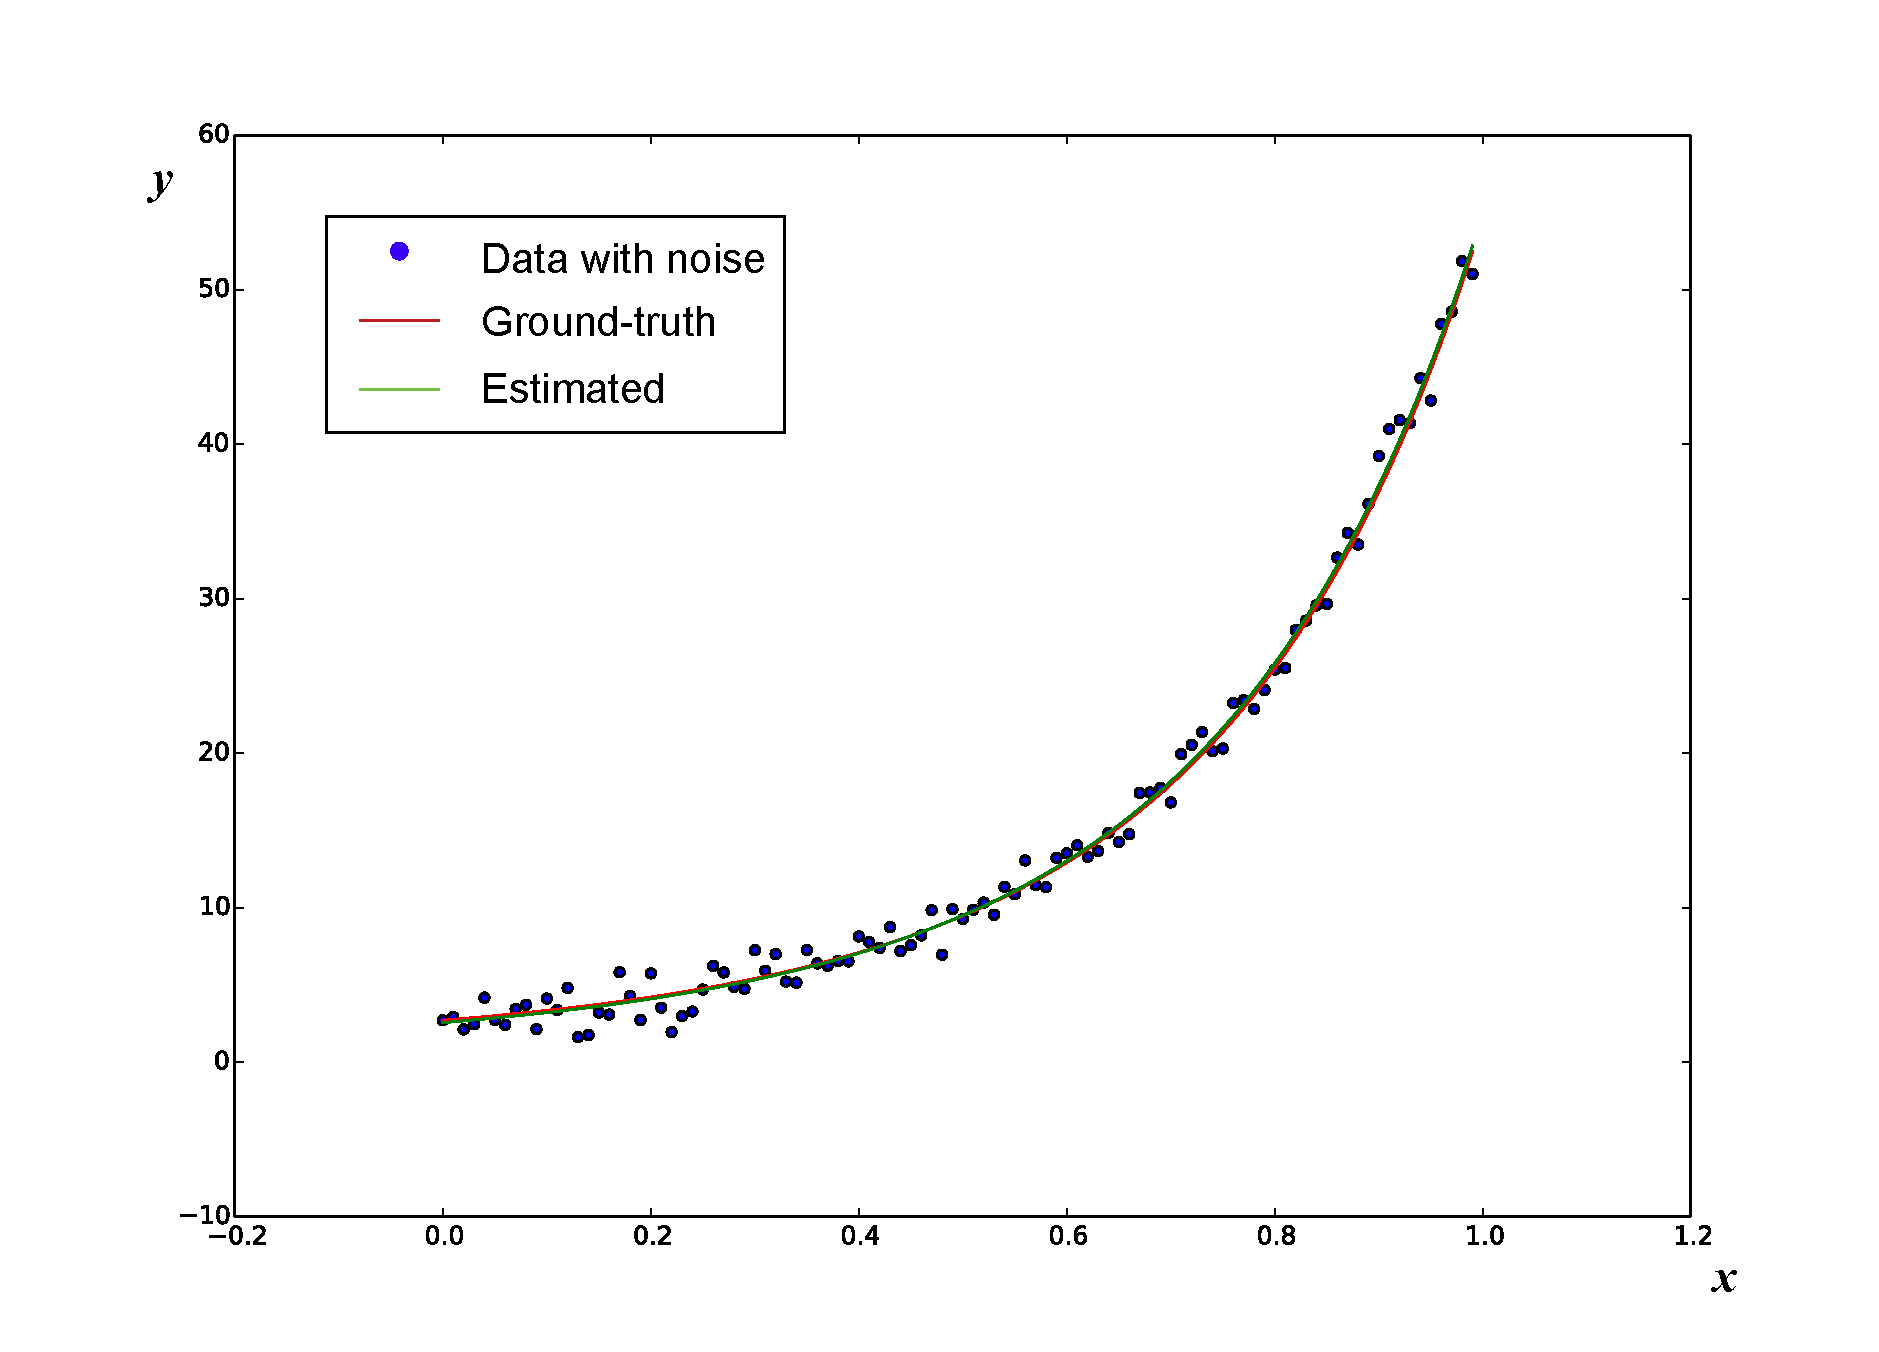
\includegraphics[width=0.8\textwidth]{optimization/ceresFitting.pdf}
    \caption{噪声$\sigma=1$时的曲线拟合结果。真实模型和估计模型非常接近。}
    \label{fig:ceres-fitting}
\end{figure}

\subsection{使用Ceres进行曲线拟合}
本节向大家介绍两个C++的优化库:来自谷歌的Ceres库\textsuperscript{\cite{Ceres}}以及基于图优化的g2o库\textsuperscript{\cite{Kummerle2011}}。由于g2o的使用还需要介绍一点图优化的相关知识,所以我们先来介绍Ceres,然后介绍一些图优化理论,最后来讲g2o。由于优化算法在之后的“视觉里程计”和“后端”中都会出现,所以请读者务必掌握优化算法的意义,理解程序的内容。

\subsubsection{Ceres简介}
Google Ceres是一个广泛使用的最小二乘问题求解库。在Ceres中,我们作为用户,只需按照一定步骤定义待解的优化问题,然后交给求解器计算即可。Ceres求解的最小二乘问题最一般的形式如下(带边界的核函数最小二乘):
\begin{equation}
\begin{array}{ll}
\min \limits_x \quad & \frac{1}{2}\sum\limits_i {{\rho _i}\left( {{{\left\| {{f_i}\left( {{x_{{i_1}}}, \cdots {x_{{i_n}}}} \right)} \right\|}^2}} \right)} \\
\mathrm{s.t.} \quad & {l_j} \leqslant {x_j} \leqslant {u_j}.
\end{array}
\end{equation}

在这个问题中,$x_1, \cdots, x_n$为优化变量,又称\textbf{参数块}(Parameter blocks),$f_i$称为\textbf{代价函数}(Cost function),也称为残差块(Residual blocks),在SLAM中亦可理解为误差项。$l_j$和$u_j$为第$j$个优化变量的上限和下限。在最简单的情况下,取$l_j = -\infty, u_j=\infty$(不限制优化变量的边界)。此时,目标函数由许多平方项经过一个\textbf{核函数}$\rho(\cdot)$之后求和组成\footnote{核函数的详细讨论见第9讲。}。同样,可以取$\rho$为恒等函数,那么目标函数即为许多项的平方和,我们就得到了无约束的最小二乘问题,和先前介绍的理论是一致的。

为了让Ceres帮我们求解这个问题,我们需要做以下几件事:
\begin{enumerate}
\item 定义每个参数块。参数块通常为平凡的向量,但是在SLAM里也可以定义成四元数、李代数这种特殊的结构。如果是向量,那么我们需要为每个参数块分配一个double数组,来存储变量的值。
\item 然后,定义残差块的计算方式。残差块通常关联若干个参数块,对它们进行一些自定义的计算,然后返回残差值。Ceres对它们求平方和之后,作为目标函数的值。
\item 残差块往往也需要定义雅可比的计算方式。在Ceres中,你可以使用它提供的“自动求导”功能,也可以手动指定雅可比的计算过程。如果要使用自动求导,那么残差块需要按照特定的写法来书写:残差的计算过程应该是一个带模板的括号运算符。这一点我们通过例子来说明。
\item 最后,把所有的参数块和残差块加入Ceres定义的Problem对象中,调用Solve函数求解即可。求解之前,我们可以传入一些配置信息,例如迭代次数、终止条件等,也可以使用默认的配置。
\end{enumerate}
下面,我们来实际操作一下Ceres求解曲线拟合问题,理解优化的过程。

\subsubsection{安装Ceres}
为了使用Ceres,我们需要对它进行编译安装。Ceres的github地址为:\url{https://github.com/ceres-solver/ceres-solver},不过你也可以直接使用本书代码3rdparty目录里的Ceres,这样你将和我使用完全一样的版本。

与之前碰到的库一样,Ceres是一个cmake工程。先来安装它的依赖项,在Ubuntu中可以用apt-get安装,主要是谷歌自己使用的一些日志和测试工具:
\begin{lstlisting}[language=sh,caption=终端输入:]
sudo apt-get install liblapack-dev libsuitesparse-dev libcxsparse3 libgflags-dev libgoogle-glog-dev libgtest-dev 
\end{lstlisting}

然后,进入Ceres库目录下,使用cmake编译并安装它。这个过程我们已经做过很多遍了,此处不再赘述。安装完成后,在/usr/local/include/ceres下找到Ceres的头文件,并在/usr/local/lib/下找到名为libceres.a的库文件。有了这些文件,就可以使用Ceres进行优化计算了。

\subsubsection{使用Ceres拟合曲线}
下面的代码演示了如何使用Ceres求解同样的问题。

\begin{lstlisting}[language=c++,caption=slambook/ch6/ceresCurveFitting.cpp]
#include <iostream>
#include <opencv2/core/core.hpp>
#include <ceres/ceres.h>
#include <chrono>

using namespace std;

// 代价函数的计算模型
struct CURVE_FITTING_COST {
    CURVE_FITTING_COST(double x, double y) : _x(x), _y(y) {}
    
    // 残差的计算
    template<typename T>
    bool operator()(
        const T *const abc, // 模型参数,有3维
        T *residual) const {
        // y-exp(ax^2+bx+c)
        residual[0] = T(_y) - ceres::exp(abc[0] * T(_x) * T(_x) + abc[1] * T(_x) + abc[2]);
        return true;
    }
    
    const double _x, _y;    // x,y数据
};

int main(int argc, char **argv) {
    double ar = 1.0, br = 2.0, cr = 1.0;         // 真实参数值
    double ae = 2.0, be = -1.0, ce = 5.0;        // 估计参数值
    int N = 100;                                 // 数据点
    double w_sigma = 1.0;                        // 噪声Sigma值
    double inv_sigma = 1.0 / w_sigma;
    cv::RNG rng;                                 // OpenCV随机数产生器
    
    vector<double> x_data, y_data;      // 数据
    for (int i = 0; i < N; i++) {
        double x = i / 100.0;
        x_data.push_back(x);
        y_data.push_back(exp(ar * x * x + br * x + cr) + rng.gaussian(w_sigma * w_sigma));
    }
    
    double abc[3] = {ae, be, ce};
    
    // 构建最小二乘问题
    ceres::Problem problem;
    for (int i = 0; i < N; i++) {
        problem.AddResidualBlock(     // 向问题中添加误差项
            // 使用自动求导,模板参数:误差类型,输出维度,输入维度,维数要与前面struct中一致
            new ceres::AutoDiffCostFunction<CURVE_FITTING_COST, 1, 3>(
                new CURVE_FITTING_COST(x_data[i], y_data[i])
            ),
            nullptr,            // 核函数,这里不使用,为空
            abc                 // 待估计参数
        );
    }
    
    // 配置求解器
    ceres::Solver::Options options;     // 这里有很多配置项可以填
    options.linear_solver_type = ceres::DENSE_NORMAL_CHOLESKY;  // 增量方程如何求解
    options.minimizer_progress_to_stdout = true;   // 输出到cout
    
    ceres::Solver::Summary summary;                // 优化信息
    chrono::steady_clock::time_point t1 = chrono::steady_clock::now();
    ceres::Solve(options, &problem, &summary);  // 开始优化
    chrono::steady_clock::time_point t2 = chrono::steady_clock::now();
    chrono::duration<double> time_used = chrono::duration_cast<chrono::duration<double>>(t2 - t1);
    cout << "solve time cost = " << time_used.count() << " seconds. " << endl;
    
    // 输出结果
    cout << summary.BriefReport() << endl;
    cout << "estimated a,b,c = ";
    for (auto a:abc) cout << a << " ";
    cout << endl;
    
    return 0;
}
\end{lstlisting}

程序中需要说明的地方均已加注释。可以看到,我们利用OpenCV的噪声生成器生成了100个带高斯噪声的数据,随后利用Ceres进行拟合。这里演示的Ceres用法有如下几项:

\begin{enumerate}
	\item 定义残差块的类。方法是书写一个类(或结构体),并在类中定义带模板参数的()运算符,这样该类就成为了一个\textbf{拟函数}(Functor)\footnote{C++术语,因为带有括号运算符的类在使用括号算符时,就仿佛是一个函数一样。}。这种定义方式使得Ceres可以像调用函数一样,对该类的某个对象(比如a)调用a<double>()方法。事实上,Ceres会把雅可比矩阵作为类型参数传入此函数,从而实现自动求导的功能。
	\item 程序中的double abc[3]即为参数块,而对于残差块,我们对每一个数据构造CURVE\_FITTING\_COST对象,然后调用AddResidualBlock将误差项添加到目标函数中。由于优化需要梯度,我们有若干种选择:(1)使用Ceres的自动求导(Auto Diff);(2)使用数值求导(Numeric Diff)\footnote{自动求导也是用数值导数实现的,但由于是模板运算,所以运行更快一些。};(3)自行推导解析的导数形式,提供给Ceres。因为自动求导在编码上是最方便的,于是我们使用自动求导。
	\item 自动求导需要指定误差项和优化变量的维度。这里的误差是标量,维度为1;优化的是$a,b,c$三个量,维度为3。于是,在自动求导类AutoDiffCostFunction的模板参数中设定变量维度为1、3。
	\item 设定好问题后,调用Solve函数进行求解。你可以在options里配置(非常详细的)优化选项。例如,可以选择使用Line Search还是Trust Region、迭代次数、步长,等等。读者可以查看Options的定义,看看有哪些优化方法可选,当然默认的配置已经可用于很广泛的问题了。
\end{enumerate}

最后,我们来看看实验结果。调用build/ceresCurveFitting查看优化结果:
\begin{lstlisting}
iter      cost      cost_change  |gradient|   |step|    tr_ratio  tr_radius  ls_iter  iter_time  total_time
0  1.597873e+06    0.00e+00    3.52e+06   0.00e+00   0.00e+00  1.00e+04        0    2.10e-05    7.92e-05
1  1.884440e+05    1.41e+06    4.86e+05   9.88e-01   8.82e-01  1.81e+04        1    5.60e-05    1.05e-03
2  1.784821e+04    1.71e+05    6.78e+04   9.89e-01   9.06e-01  3.87e+04        1    2.00e-05    1.09e-03
3  1.099631e+03    1.67e+04    8.58e+03   1.10e+00   9.41e-01  1.16e+05        1    6.70e-05    1.16e-03
4  8.784938e+01    1.01e+03    6.53e+02   1.51e+00   9.67e-01  3.48e+05        1    1.88e-05    1.19e-03
5  5.141230e+01    3.64e+01    2.72e+01   1.13e+00   9.90e-01  1.05e+06        1    1.81e-05    1.22e-03
6  5.096862e+01    4.44e-01    4.27e-01   1.89e-01   9.98e-01  3.14e+06        1    1.79e-05    1.25e-03
7  5.096851e+01    1.10e-04    9.53e-04   2.84e-03   9.99e-01  9.41e+06        1    1.81e-05    1.28e-03
solve time cost = 0.00130755 seconds. 
Ceres Solver Report: Iterations: 8, Initial cost: 1.597873e+06, Final cost: 5.096851e+01, Termination: CONVERGENCE
estimated a,b,c = 0.890908 2.1719 0.943628 
\end{lstlisting}

最终的优化值和我们上一节的实验结果基本相同,但运行速度上Ceres要相对慢一些。在我的机器上Ceres约使用了1.3个毫秒,这比手写高斯牛顿法慢了约六倍左右。

希望读者通过这个简单的例子对Ceres的使用方法有一个大致了解。它的优点是提供了自动求导工具,使得不必去计算很麻烦的雅可比矩阵。Ceres的自动求导是通过模板元实现的,在编译时期就可以完成自动求导工作,不过仍然是数值导数。本书大部分时候仍然会介绍雅可比矩阵的计算,因为那样对理解问题更有帮助,而且在优化中更少出现问题。此外,Ceres的优化过程配置也很丰富,使其适合很广泛的最小二乘优化问题,包括SLAM之外的各种问题。

\subsection{使用g2o进行曲线拟合}
本讲的第2个实践部分将介绍另一个(主要在SLAM领域)广为使用的优化库:g2o(General Graphic Optimization,G$^2$O)。它是一个基于\textbf{图优化}的库。图优化是一种将非线性优化与图论结合起来的理论,因此在使用它之前,我们花一点篇幅介绍一下图优化理论。

\subsubsection{图优化理论简介}
我们已经介绍了非线性最小二乘的求解方式。它们是由很多个误差项之和组成的。然而,仅有一组优化变量和许多个误差项,我们并不清楚它们之间的\textbf{关联}。比如,某个优化变量$x_j$存在于多少个误差项中呢?我们能保证对它的优化是有意义的吗?进一步,我们希望能够直观地看到该优化问题\textbf{长什么样}。于是,就牵涉到了图优化。

图优化,是把优化问题表现成\textbf{图(Graph)}的一种方式。这里的\textbf{图}是图论意义上的图。一个图由若干个\textbf{顶点(Vertex)},以及连接着这些顶点的\textbf{边(Edge)}组成。进而,用\textbf{顶点}表示\textbf{优化变量},用\textbf{边}表示\textbf{误差项}。于是,对任意一个上述形式的非线性最小二乘问题,我们可以构建与之对应的一个\textbf{图}。我们可以简单地称它为\textbf{图},也可以用概率图里的定义,称之为\textbf{贝叶斯图}或\textbf{因子图}。

\autoref{fig:graph-optimization}~是一个简单的图优化例子。我们用三角形表示相机位姿节点,用圆形表示路标点,它们构成了图优化的顶点;同时,实线表示相机的运动模型,虚线表示观测模型,它们构成了图优化的边。此时,虽然整个问题的数学形式仍是式\eqref{eq:least-square}那样,但现在我们可以直观地看到问题的\textbf{结构}了。如果希望,也可以做\textbf{去掉孤立顶点}或\textbf{优先优化边数较多(或按图论的术语,度数较大)的顶点}这样的改进。但是最基本的图优化是用图模型来表达一个非线性最小二乘的优化问题。而我们可以利用图模型的某些性质做更好的优化。

\begin{figure}[!ht]
	\centering
	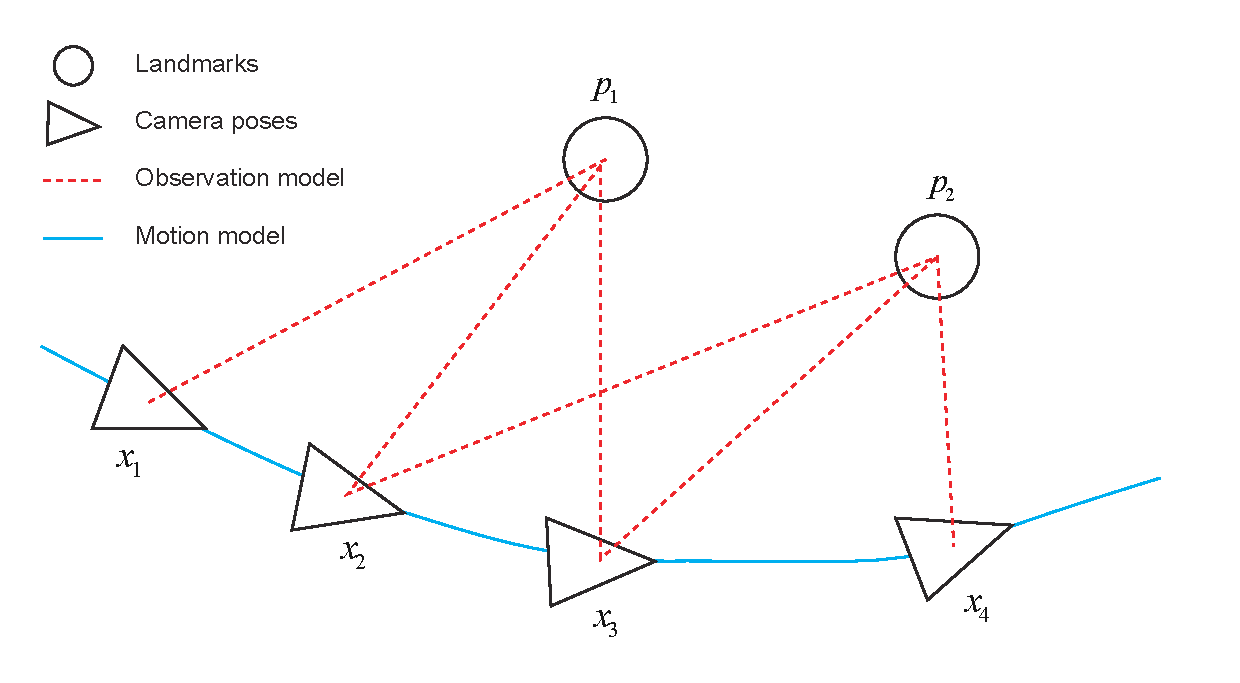
\includegraphics[width=1.0\textwidth]{Optimization/graphOptimization.pdf}
	\caption{图优化的例子。}
	\label{fig:graph-optimization}
\end{figure}

g2o是一个通用的图优化库。“通用”意味着你可以在g2o里求解任何能够表示为图优化的最小二乘问题,显然包括上面谈的曲线拟合问题。下面我们来演示这个过程。

\subsection{g2o的编译与安装}
在使用一个库之前,我们需要对它进行编译和安装。读者应该已经体验过很多次这种过程了,它们基本大同小异。关于g2o,读者可以从GitHub下载它:\url{https://github.com/RainerKuemmerle/g2o},或从本书提供的第三方代码库中获得。由于g2o还在继续更新,所以我建议你使用3rdparty下的g2o以保证版本与我的相同。

g2o也是一个cmake工程。我们先来安装它的依赖项(部分依赖项与Ceres重合):
\begin{lstlisting}[language=sh,caption=终端输入:]
sudo apt-get install qt5-qmake qt5-default libqglviewer-dev-qt5 libsuitesparse-dev libcxsparse3 libcholmod3
\end{lstlisting}

然后,按照cmake的方式对g2o进行编译安装即可,这里略去对该过程的说明。安装完成后,g2o的头文件将位于/usr/local/g2o下,库文件位于/usr/local/lib/下。现在,我们重新考虑Ceres例程中的曲线拟合实验,在g2o中实验一遍。

\subsection{使用g2o拟合曲线}
为了使用g2o,首先要将曲线拟合问题抽象成图优化。这个过程中,只要记住\textbf{节点为优化变量,边为误差项}即可。曲线拟合的图优化问题可以画成\autoref{fig:graph-fitting}~的形式。

\begin{figure}[!ht]
	\centering
	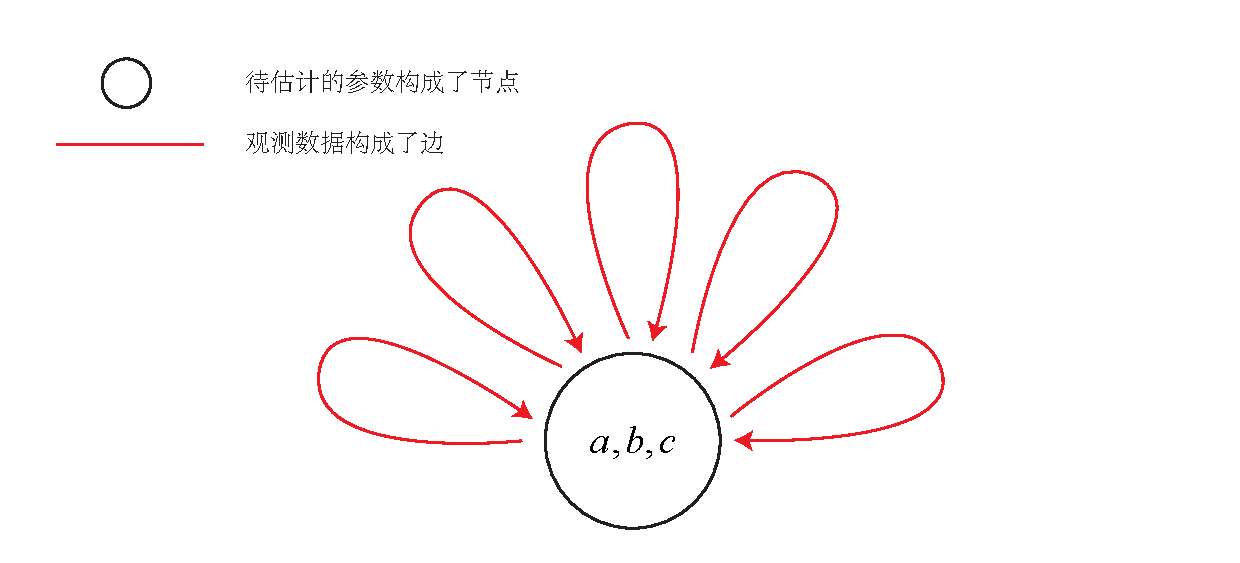
\includegraphics[width=.9\textwidth]{Optimization/graphFitting.pdf}
	\caption{曲线拟合对应的图优化模型。(莫明其妙地有些像华为的标志)}
	\label{fig:graph-fitting}
\end{figure}

在曲线拟合问题中,整个问题只有一个顶点:曲线模型的参数$a,b,c$;而各个带噪声的数据点,构成了一个个误差项,也就是图优化的边。但这里的边与我们平时想的边不太一样,它们是\textbf{一元边}(Unary Edge),即\textbf{只连接一个顶点}——因为整个图只有一个顶点。所以在\autoref{fig:graph-fitting}~中,我们只能把它画成自己连到自己的样子。事实上,图优化中一条边可以连接一个、两个或多个顶点,这主要反映每个误差与多少个优化变量有关。在稍有些玄妙的说法中,我们把它叫作\textbf{超边}(Hyper Edge),整个图叫作\textbf{超图}(Hyper Graph)\footnote{显然我个人并不太喜欢有些故弄玄虚的说法,我是个自然主义者。}。

弄清了这个图模型之后,接下来就是在g2o中建立该模型进行优化了。作为g2o的用户,我们要做的事主要包含以下步骤:

\begin{enumerate}
	\item 定义顶点和边的类型。
	\item 构建图。
	\item 选择优化算法。
	\item 调用g2o进行优化,返回结果。
\end{enumerate}

这部分和Ceres是非常相似的,当然程序在书写上会有一些不同。下面演示一下程序。

\begin{lstlisting}[language=c++,caption=slambook/ch6/g2oCurveFitting.cpp]
#include <iostream>
#include <g2o/core/g2o_core_api.h>
#include <g2o/core/base_vertex.h>
#include <g2o/core/base_unary_edge.h>
#include <g2o/core/block_solver.h>
#include <g2o/core/optimization_algorithm_levenberg.h>
#include <g2o/core/optimization_algorithm_gauss_newton.h>
#include <g2o/core/optimization_algorithm_dogleg.h>
#include <g2o/solvers/dense/linear_solver_dense.h>
#include <Eigen/Core>
#include <opencv2/core/core.hpp>
#include <cmath>
#include <chrono>

using namespace std;

// 曲线模型的顶点,模板参数:优化变量维度和数据类型
class CurveFittingVertex : public g2o::BaseVertex<3, Eigen::Vector3d> {
public:
    EIGEN_MAKE_ALIGNED_OPERATOR_NEW
    
    // 重置
    virtual void setToOriginImpl() override {
        _estimate << 0, 0, 0;
    }
    
    // 更新
    virtual void oplusImpl(const double *update) override {
        _estimate += Eigen::Vector3d(update);
    }
    
    // 存盘和读盘:留空
    virtual bool read(istream &in) {}
    virtual bool write(ostream &out) const {}
};

// 误差模型 模板参数:观测值维度,类型,连接顶点类型
class CurveFittingEdge : public g2o::BaseUnaryEdge<1, double, CurveFittingVertex> {
public:
    EIGEN_MAKE_ALIGNED_OPERATOR_NEW
    
    CurveFittingEdge(double x) : BaseUnaryEdge(), _x(x) {}
    
    // 计算曲线模型误差
    virtual void computeError() override {
        const CurveFittingVertex *v = static_cast<const CurveFittingVertex *> (_vertices[0]);
        const Eigen::Vector3d abc = v->estimate();
        _error(0, 0) = _measurement - std::exp(abc(0, 0) * _x * _x + abc(1, 0) * _x + abc(2, 0));
    }
    
    // 计算雅可比矩阵
    virtual void linearizeOplus() override {
        const CurveFittingVertex *v = static_cast<const CurveFittingVertex *> (_vertices[0]);
        const Eigen::Vector3d abc = v->estimate();
        double y = exp(abc[0] * _x * _x + abc[1] * _x + abc[2]);
        _jacobianOplusXi[0] = -_x * _x * y;
        _jacobianOplusXi[1] = -_x * y;
        _jacobianOplusXi[2] = -y;
    }
    
    virtual bool read(istream &in) {}
    virtual bool write(ostream &out) const {}
public:
    double _x;  // x 值, y 值为 _measurement
};

int main(int argc, char **argv) {
    // 省略数据生成部分代码
    // 构建图优化,先设定g2o
    typedef g2o::BlockSolver<g2o::BlockSolverTraits<3, 1>> BlockSolverType;  // 每个误差项优化变量维度为3,误差值维度为1
    typedef g2o::LinearSolverDense<BlockSolverType::PoseMatrixType> LinearSolverType; // 线性求解器类型
    
    // 梯度下降方法,可以从GN, LM, DogLeg 中选
    auto solver = new g2o::OptimizationAlgorithmGaussNewton(
        g2o::make_unique<BlockSolverType>(g2o::make_unique<LinearSolverType>()));
    g2o::SparseOptimizer optimizer;     // 图模型
    optimizer.setAlgorithm(solver);   // 设置求解器
    optimizer.setVerbose(true);       // 打开调试输出
    
    // 往图中增加顶点
    CurveFittingVertex *v = new CurveFittingVertex();
    v->setEstimate(Eigen::Vector3d(ae, be, ce));
    v->setId(0);
    optimizer.addVertex(v);
    
    // 往图中增加边
    for (int i = 0; i < N; i++) {
        CurveFittingEdge *edge = new CurveFittingEdge(x_data[i]);
        edge->setId(i);
        edge->setVertex(0, v);                // 设置连接的顶点
        edge->setMeasurement(y_data[i]);      // 观测数值
        edge->setInformation(Eigen::Matrix<double, 1, 1>::Identity() * 1 / (w_sigma * w_sigma)); // 信息矩阵:协方差矩阵之逆
        optimizer.addEdge(edge);
    }
    
    // 执行优化
    cout << "start optimization" << endl;
    chrono::steady_clock::time_point t1 = chrono::steady_clock::now();
    optimizer.initializeOptimization();
    optimizer.optimize(10);
    chrono::steady_clock::time_point t2 = chrono::steady_clock::now();
    chrono::duration<double> time_used = chrono::duration_cast<chrono::duration<double>>(t2 - t1);
    cout << "solve time cost = " << time_used.count() << " seconds. " << endl;
    
    // 输出优化值
    Eigen::Vector3d abc_estimate = v->estimate();
    cout << "estimated model: " << abc_estimate.transpose() << endl;
    
    return 0;
}
\end{lstlisting}

在这个程序中,我们从g2o派生出了用于曲线拟合的图优化顶点和边:CurveFittingVertex和CurveFittingEdge,这实质上扩展了g2o的使用方式。这两个类分别派生自BaseVertex和BaseUnaryEdge类。在派生类中,我们重写了重要的虚函数:

\begin{enumerate}
	\item 顶点的更新函数:oplusImpl。我们知道优化过程最重要的是增量$\Delta \bm{x}$的计算,而该函数处理的是$\bm{x}_{k+1} = \bm{x}_k + \Delta \bm{x}$的过程。
	
	读者也许觉得这并不是什么值得一提的事情,因为仅仅是个简单的加法而已,为什么g2o不帮我们完成呢?在曲线拟合过程中,由于优化变量(曲线参数)本身位于\textbf{向量空间}中,这个更新计算确实就是简单的加法。但是,当优化变量不在向量空间中时,比如说$\bm{x}$是相机位姿,它本身不一定有加法运算。这时,就需要重新定义\textbf{增量如何加到现有的估计上}的行为了。按照第4讲的解释,我们可能使用左乘更新或右乘更新,而不是直接的加法。
	
	\item 顶点的重置函数:setToOriginImpl。这是平凡的,我们把估计值置零即可。
	
	\item 边的误差计算函数:computeError。该函数需要取出边所连接的顶点的当前估计值,根据曲线模型,与它的观测值进行比较。这和最小二乘问题中的误差模型是一致的。
    
    \item 边的雅可比计算函数:linearizeOplus。这个函数里我们计算了每条边相对于顶点的雅可比。
	
	\item 存盘和读盘函数:read、write。由于我们并不想进行读/写操作,所以留空。
\end{enumerate}

定义了顶点和边之后,我们在main函数里声明了一个图模型,然后按照生成的噪声数据,往图模型中添加顶点和边,最后调用优化函数进行优化。g2o会给出优化的结果:

\clearpage
\begin{lstlisting}[language=sh,caption=终端输出:]
start optimization
iteration= 0	 chi2= 376785.128234	 time= 3.3299e-05	 cumTime= 3.3299e-05	 edges= 100	 schur= 0
iteration= 1	 chi2= 35673.566018	 time= 1.3789e-05	 cumTime= 4.7088e-05	 edges= 100	 schur= 0
iteration= 2	 chi2= 2195.012304	 time= 1.2323e-05	 cumTime= 5.9411e-05	 edges= 100	 schur= 0
iteration= 3	 chi2= 174.853126	 time= 1.3302e-05	 cumTime= 7.2713e-05	 edges= 100	 schur= 0
iteration= 4	 chi2= 102.779695	 time= 1.2424e-05	 cumTime= 8.5137e-05	 edges= 100	 schur= 0
iteration= 5	 chi2= 101.937194	 time= 1.2523e-05	 cumTime= 9.766e-05	 edges= 100	 schur= 0
iteration= 6	 chi2= 101.937020	 time= 1.2268e-05	 cumTime= 0.000109928	 edges= 100	 schur= 0
iteration= 7	 chi2= 101.937020	 time= 1.2612e-05	 cumTime= 0.00012254	 edges= 100	 schur= 0
iteration= 8	 chi2= 101.937020	 time= 1.2159e-05	 cumTime= 0.000134699	 edges= 100	 schur= 0
iteration= 9	 chi2= 101.937020	 time= 1.2688e-05	 cumTime= 0.000147387	 edges= 100	 schur= 0
solve time cost = 0.000919301 seconds. 
estimated model: 0.890912   2.1719 0.943629
\end{lstlisting}

我们使用高斯—牛顿方法进行梯度下降,在迭代了9次后得到优化结果,与Ceres和手写高斯牛顿法相差无几。从运行速度来看,我们实验结论是手写快于g2o,而g2o快于Ceres。这是一个大体符合直觉的经验,通用性和高效性往往是互相矛盾的。但是本实验中Ceres使用了自动求导,且求解器配置与高斯牛顿还不完全一致,所以看起来慢一些。

\section{小结}
本节介绍了SLAM中经常碰到的一种非线性优化问题:由许多个误差项平方和组成的最小二乘问题。我们介绍了它的定义和求解,并且讨论了两种主要的梯度下降方式:高斯牛顿法和列文伯格—马夸尔特方法。在实践部分中,分别使用了手写高斯牛顿法、Ceres和g2o两种优化库求解同一个曲线拟合问题,发现它们给出了相似的结果。

由于还没有详细谈Bundle Adjustment,所以我们在实践部分选择了曲线拟合这样一个简单但有代表性的例子,以演示一般的非线性最小二乘求解方式。特别地,如果用g2o来拟合曲线,必须先把问题转换为图优化,定义新的顶点和边,这种做法是有一些迂回的——g2o的主要目的并不在此。相比之下,Ceres定义误差项求曲线拟合问题则自然了很多,因为它本身即是一个优化库。然而,在SLAM中更多的问题是,一个带有许多个相机位姿和许多个空间点的优化问题如何求解。特别地,当相机位姿以李代数表示时,误差项关于相机位姿的导数如何计算,将是一件值得详细讨论的事。我们将在后续内容发现,g2o提供了大量现成的顶点和边,非常便于相机位姿估计问题。而在Ceres中,我们不得不自己实现每一个Cost Function,有一些不便。

在实践部分的两个程序中,我们没有去计算曲线模型关于三个参数的导数,而是利用了优化库的数值求导,这使得理论和代码都会简洁一些。Ceres库提供了基于模板元的自动求导和运行时的数值求导,而g2o只提供了运行时数值求导这一种方式。但是,对于大多数问题,如果能够推导出雅可比矩阵的解析形式并告诉优化库,就可以避免数值求导中的诸多问题。

最后,希望读者能够适应Ceres和g2o这些大量使用模板编程的方式。也许一开始会看上去比较吓人(特别是Ceres设置残差块的括号运算符,以及g2o初始化部分的代码),但是熟悉之后,就会觉得这样的方式是自然的,而且容易扩展。我们将在SLAM后端一讲中继续讨论稀疏性、核函数、位姿图(Pose Graph)等问题。

\section*{习题}
\begin{enumerate}
	\item 证明线性方程$\bm{A} \bm{x} = \bm{b}$当系数矩阵$\bm{A}$超定时,最小二乘解为$\bm{x} = (\bm{A}^\mathrm{T}\bm{A})^{-1}\bm{A}^\mathrm{T} \bm{b}$。
	\item 调研最速下降法、牛顿法、高斯牛顿法和列文伯格—马夸尔特方法各有什么优缺点。除了我们举的Ceres库和g2o库,还有哪些常用的优化库?(你可能会找到一些MATLAB上的库。)
	\item 为什么高斯牛顿法的增量方程系数矩阵可能不正定?不正定有什么几何含义?为什么在这种情况下解就不稳定了?
	\item DogLeg是什么?它与高斯牛顿法和列文伯格—马夸尔特方法有何异同?请搜索相关的材料\footnote{\mbox{例如,}\url{http://www.numerical.rl.ac.uk/people/nimg/course/lectures/raphael/lectures/lec7slides.pdf}。}。
	\item 阅读Ceres的教学材料(\url{http://ceres-solver.org/tutorial.html})以更好地掌握其用法。
	\item 阅读g2o自带的文档,你能看懂它吗?如果还不能完全看懂,请在第10讲和第11讲之后回来再看。
	\item[\optional] 请更改曲线拟合实验中的曲线模型,并用Ceres和g2o进行优化实验。例如,可以使用更多的参数和更复杂的模型。
\end{enumerate}
